\newpage
\section {Билет 15. Модели взаимодействия, ошибок, безопасности.}

Различные архитектуры распределённых систем имеют много общего.\\
\textbf{1. Модели взаимодействия}
\begin{itemize}
\item Характеристики коммуникационного канала:

Пропускная способность, 

задержка при передаче пакета - зависит от физической структуры и количества промежуточных структур, 

jitter - изменение величины задержки при передаче последовательности пакетов, каждый кконкретный пакет передается быстрее или медленнее. 

\item Упорядочивание сообщений.

Причинно-следственный порядок. Мы можем спокойно сравнивать время события в одном процессе, но между разными процессами можно сравнивать только при наличии передачи сообщения, так как нельзя получить ообщение раньше, чем оно было отправленно.

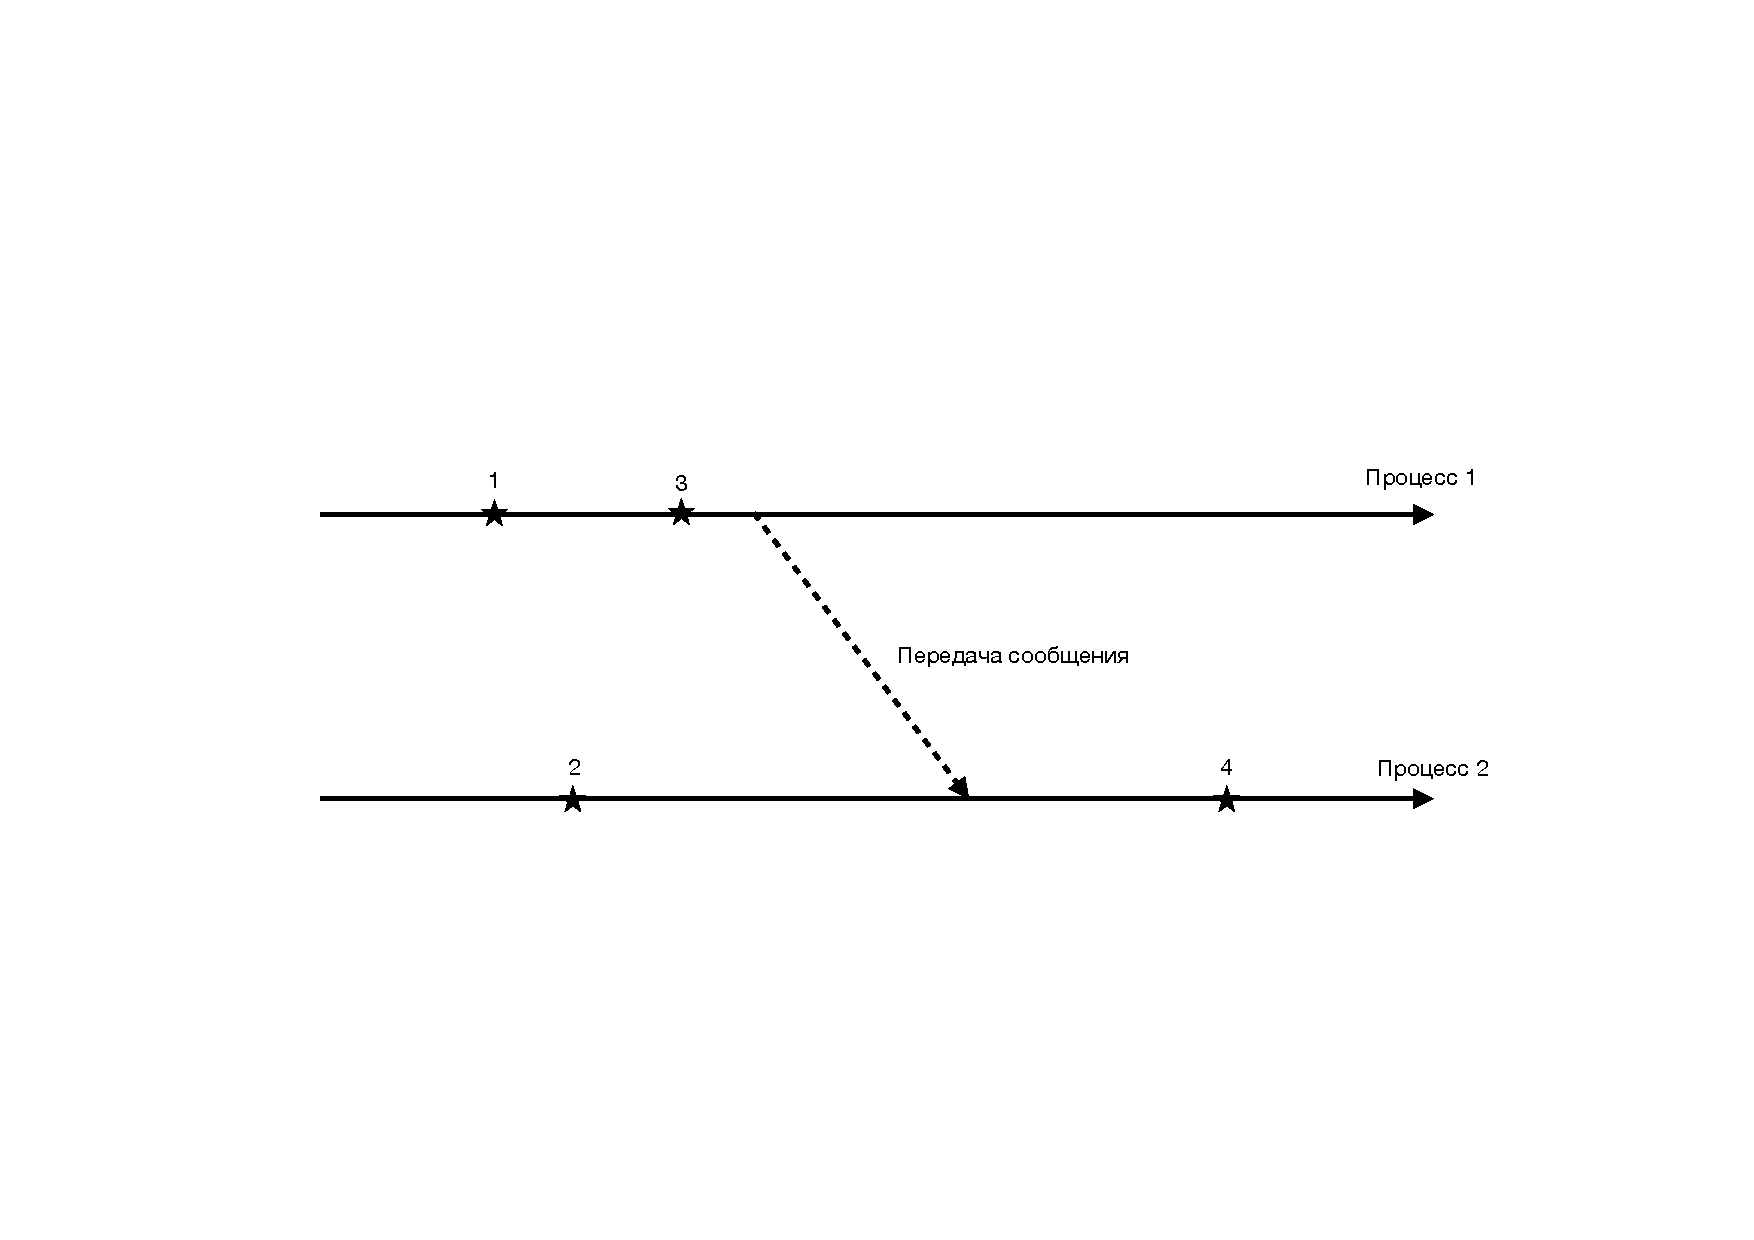
\includegraphics[scale=0.7]{15/masseg_time.pdf}

Так, на картинке, процесс 2 знает порядок временных меток в процессе 1 до передачи сообщения (1 и 3) и знает что они все были до метки 4, но сравнить порядок 1 или 3 с меткой 2 нельзя, так в распределённой системе отсутствуют глобальные часы и сиинхронизировать процессы нельзя.
 
 Более подробно этот пункт разобран в билете 20.
 
\item  Синхронные и асинхронные системы.

В синхронных мы знаем точное время задержки (если пакет не был доставлен за какое-то время, то он не будет доставлен никогда), и знаем время ответа другого узла (выполнения операции).

В асинхронных системах не знаем ничего, модель менее удобная, но более жизненная.
\end{itemize} 
\textbf{\noindent 2. Модели ошибок}

Процесс может работать до какого-то момента, после чего отказать и далее:\\
 \textit{Наблюдаемый отказ}  -  другие участники могут узнать, что он погиб.\\
 \textit{Ненаблюдаемый отказ}  - другие участники не могут узнать, что он погиб.\\
\textit{Потеря} (в канале) - сообщение отправленно, но не дошло. \\
\textit{Пропуск отправки} (в процессе) - не отправляет сообщения.\\
\textit{Пропуск приема} (в процессе) - не получает сообщения.\\
\textit{Произвольное поведение} (и в канале, и в процессе) - поведение, не предписанное протоколом, возникшее из-за ошибок или злоумышленно.\\
\\
\textbf{\noindent 3. Модели безопасности}
\begin{itemize}
\setlength\itemsep{0.0001em}
\item Описание информационной системы
\item Структурно-функциональные характеристики
\item Описание угроз безопасности
\item Модель нарушителя
\item Возможные уязвимости
\item Способы реализации угроз
\item Последствия от нарушения свойств безопасности информации.
\end{itemize}




